This section first presents the implementation details chosen to evaluate MSF in this paper. Then, the studied use case is presented. Once this context is clear the MSC performance is evaluated as well as both available parallelization techniques, data and task. Finally, the performance model proposed in Section~\ref{sect:perfs}.

%-------------------------------------
\subsection{Implementation details}

The two main implementation choices to take in MSC and its specialized assembly generation concern the technologies used for data and task parallelizations.

For the data-parallelization, as already detailed many times throughout the paper, a third party HPC specialist is responsible for implementing $DDS$ and $Data$ using a chosen library or external language and by following the interfaces specified by these two components. To evaluate MSF, we have played the role of HPC specialists and have implemented these components using SkelGIS, a C++ embedded DSL~\cite{CPE:CPE3494} that proposes a distributed Cartesian mesh as well as user API to manipulate structures while hiding their underlying distribution.

For the task parallelism, we have chosen to use OpenMP~\cite{660313} to generate the code of the $Scheduler$ component. OpenMP targets shared-memory platforms only. Although the version 4 of OpenMP has introduced explicit support for dynamic task scheduling, our implementation only requires version 3 whose fork-join model is well suited for the static scheduling introduced in Section~\ref{sect:parallelism}.
The use of dynamic schedulers, such as provided by libgomp\footnote{\url{https://gcc.gnu.org/projects/gomp/}}, StarPU~\cite{Augonnet2011}, or XKaapi~\cite{Gautier:2013:XRS:2510661.2511383},  to directly execute the DAG $\Gamma_{dep}$ will be the subject of future works.

As a result, the MSL compiler generates a hybrid code which uses both SkelGIS and OpenMP.
It also generates empty components where the developer must provide local sequential implementations of the kernels. In our case these kernels are written using SkelGIS API.

%-------------------------------------
\subsection{Use case description}

All evaluations presented in this section are based on a real case study of the shallow-Water Equations as solved in the FullSWOF2D\footnote{\url{http://www.univ-orleans.fr/mapmo/soft/FullSWOF/}}~\cite{Ferrari2004,CPE:CPE3494} code from the MAPMO laboratory, University of Orl\'eans.
In 2013, a full SkelGIS implementation of this use case has been performed by numericians and developers of the MAPMO laboratory~\cite{CPE:CPE3494,cordier2013fullswof,coullon:hal-00832660}. From this implementation we have kept the code of computation kernels to directly use it into $K$ components. Compared to a full SkelGIS implementation, where synchronizations and fusions are handled manually, MSF automatically compute where synchronizations are needed and how to perform a fusion without errors. To evaluate MSF on this use case we have described the FullSWOF2D simulation by using MSL. FullSWOF2D contains 3~mesh entities, 7~computation domains, 48~data and 98~computations (32~stencil kernels and 66~local kernels). Performances of the obtained implementation are compared to the full SkelGIS implementation to show that no overheads are introduced by MSF.

%-------------------------------------
\subsection{Compiler evaluation}

Table~\ref{fig:exectime} illustrates the execution time of each step of MSC for the FullSWOF2D example.
This has been computed on a laptop with a dual-core Intel Core i5 1.4~GHz, and 8~GB of DDR3.
While the overall time of 4.6 seconds remains reasonable, one can notice that the computation of the $TSP$ tree is by far the longest step.
As a matter of fact, the complexity of the algorithm for N-shapes removal is $O(n^3)$.
If this complexity is not a problem at the moment and onto this use case it could become one for just-in-time compilation or bigger simulations. The replacement of the static scheduling by a dynamic scheduling using dedicated tools (such as OpenMP 4, StarPU etc.) should solve this in the future.

\begin{table}[!h]
 \begin{center}
 \begin{tabular}{|c|c|c|c|c|}
   Step & Parser & $\Gamma_{sync}$ & $\Gamma_{dep}$ & $TSP$\\
   \hline
   Time (ms) & 1 & 2 & 4.2 & 3998.5\\
   \% & 0.022 & 0.043 & 0.09 & 86.6\\
 \end{tabular}
\caption{Execution times of the MSL compiler}
\label{fig:exectime}
 \end{center}
\end{table}

%-------------------------------------
\subsection{Data parallelism evaluation}

In this evaluation, we disable task-parallelism to focus on data-parallelism. Two versions of code are compared in this section: first a plain SkelGIS implementation of FullSWOF2D, where synchronizations and fusions are handled manually; second, the automatic synchronizations and fusions handled by MSF over SkelGIS. SkelGIS has already been evaluated in comparison with a native MPI implementation for the FullSWOF2D example~\cite{CPE:CPE3494}. For this reason, this section uses the plain SkelGIS implementation as the reference version. This enables to evaluate both the choices made by MSC as well as the potential overheads of using \llc~\cite{l2c} that is not used in the plain SkelGIS version. The evaluations have been performed on the Curie supercomputer (TGCC, France) described in Table~\ref{tab:TGCC}. Each evaluation has been performed nine times and the median is presented in results.

\begin{table}[!ht]
\begin{center}
 \begin{tabular}{|c|c|}
     & TGCC Curie Thin Nodes\\
     \hline         
    Processor & 2$\times$SandyBridge\\
    & (2.7 GHz)\\
    Cores/node & 16 \\
    RAM/node & 64 GB\\
    RAM/core & 4GB\\
    Compiler [-O3] & gcc 4.9.1\\
    MPI & Bullxmpi\\
 \end{tabular}
 \caption{\label{tab:TGCC}Hardware configuration of TGCC Curie Thin nodes.}
 \end{center}
\end{table}

Figures~\ref{fig:weak1}, \ref{fig:weak2} and~\ref{fig:weak3} respectively show weak scalings for a computation domain of $400 \times 400$ cells by core, $600 \times 600$ cells by core and $800 \times 800$ cells by core from 16 cores to 16.384 cores, as resumed in Table~\ref{tab:weak}.

\begin{table}[!ht]
\begin{center}
 \begin{tabular}{|c|c|}
    Domain size per core & Number of iterations\\
    \hline
     $400 \times 400$ & $200$\\
     $600 \times 600$ & $200$\\
     $800 \times 800$ & $200$\\
 \end{tabular}
 \caption{\label{tab:weak}Weak scaling experiments of Fig.~\ref{fig:weak1}, Fig.~\ref{fig:weak2} and Fig.~\ref{fig:weak3}.}
 \end{center}
\end{table}

\paragraph{\textbf{Weak scaling}}
\begin{figure}[t]
\begin{minipage}{.475\textwidth}
  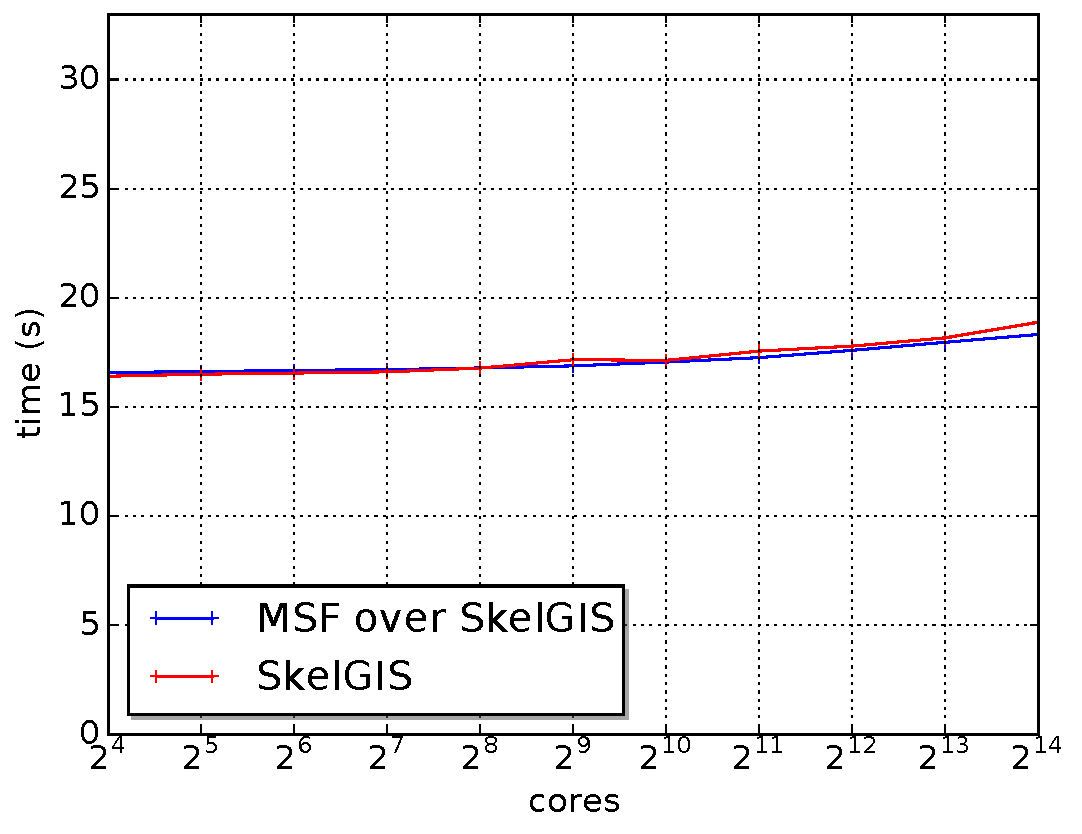
\includegraphics[width=\textwidth]{../results/weak_scaling/400_200/median_weak.pdf}
  \caption{weak-scaling with $400 \times 400$ domain per core and $200$ time iterations.}
  \label{fig:weak1}
\end{minipage}
\hfill
\begin{minipage}{.475\textwidth}
  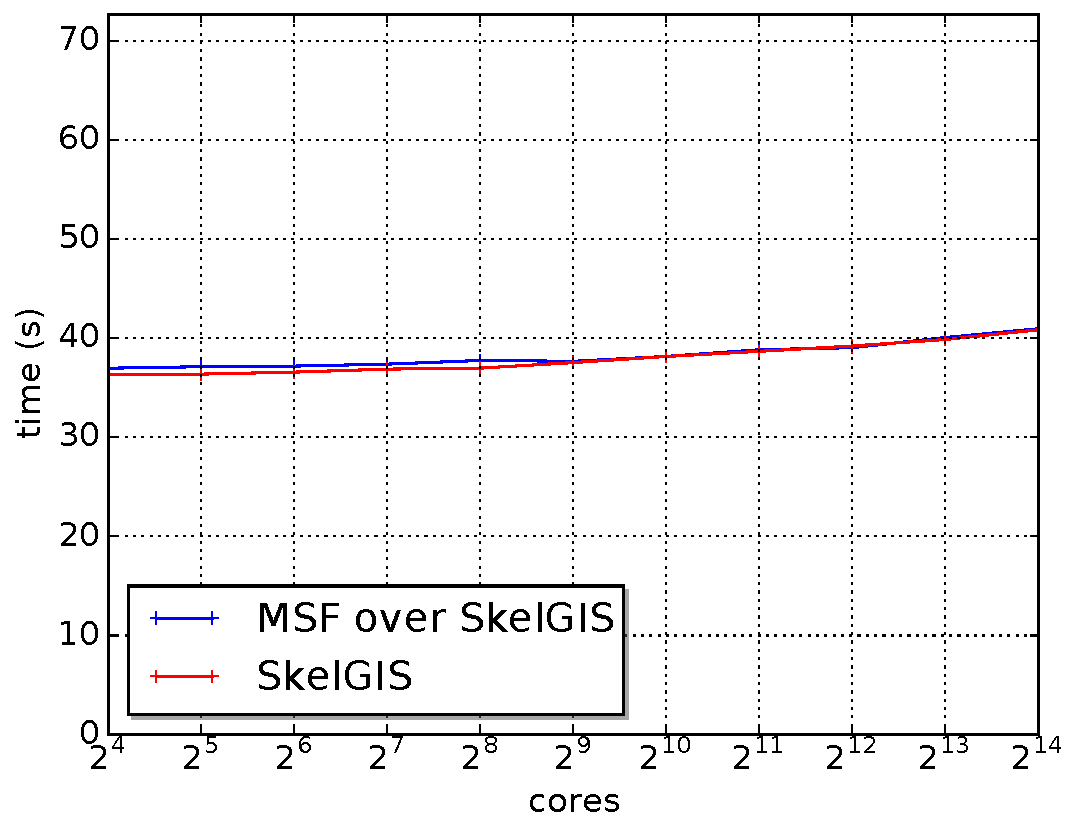
\includegraphics[width=\textwidth]{../results/weak_scaling/600_200/median_weak.pdf}
  \caption{weak-scaling with $600 \times 600$ domain per core and $200$ time iterations.}
  \label{fig:weak2}
\end{minipage}\end{figure}

\begin{figure}[t]
\begin{center}
  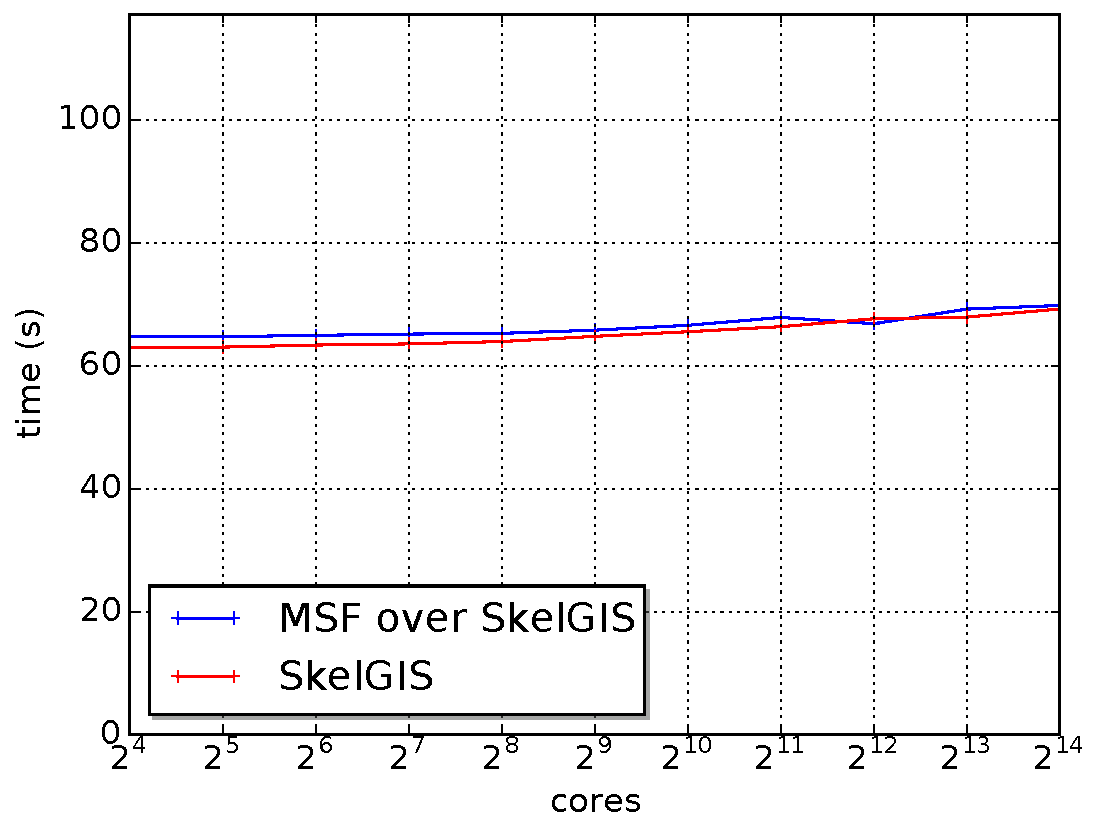
\includegraphics[width=.6\textwidth]{../results/weak_scaling/800_200/median_weak.pdf}
  \caption{weak-scaling with $800 \times 800$ domain per core and $200$ time iterations.}
  \label{fig:weak3}
 \end{center}
\end{figure}

From these results, one can notice first that performances of MSF are very close to the reference version using plain SKelGIS. This is a very good result which shows first that MSC performs good synchronizations and fusions, and second that overheads introduced by \llc are limited thanks to a good granularity in GA.
However, it seems that a slightly drop of performance happens when the domain size per core increases. This performance decrease is really small though, with a maximum difference between the two versions of 2.83\%.

The only noticeable difference between the two versions are due to \llc which load dynamic libraries at runtime. Because of this particularity, components of \llc are compiled with the \emph{-fpic} compilation flag while the SkelGIS version does not. This flag can have slight positive or negative effect on code performance depending on the situation and might be responsible for the observed difference.

%\HC{another benchmark to show that with the static version of \llc the problem disappear ?}

\paragraph{\textbf{Strong scaling}}
\begin{figure}[t]\begin{center}
  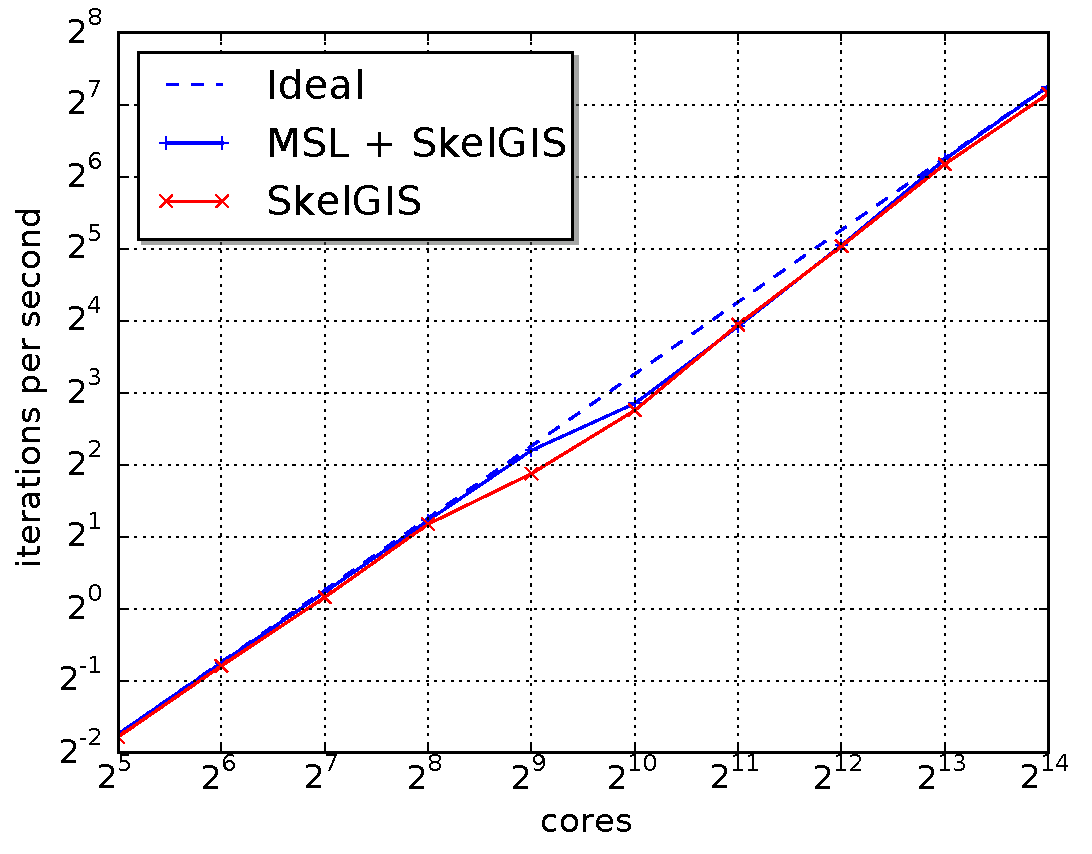
\includegraphics[width=.6\textwidth]{../results/strong_scaling/10K_1K/median_strong.pdf}
  \caption{Strong scaling on a $10k \times 10k$ domain and $1000$ time iterations.}
  \label{fig:strong}
\end{center}\end{figure}

Figure~\ref{fig:strong} shows the number of iteration per second for a 10k$\times$10k global domain size from 16 to 16.384 cores. The total number of time iterations for this benchmark is $1000$. In addition to the reference SkelGIS version, the ideal strong scaling is also illustrated in the figure.

First, one can notice that the strong scaling evaluated for the MSF version is close to the ideal speedup up to 16.384 cores, which is a very good result. Moreover, no overheads are introduced by MSF which shows that automatic synchronizations and automatic fusions are the same one that the one written manually into the plain SkelGIS version. Finally, no overheads are introduced by components of \llc. A small behavior difference can be noticed with $2^9=512$ cores, however this variation is no longer observed with 1024 cores.

%\paragraph{\textbf{Fusion}} Finally, we evaluate loop fusions automatically proposed by MSF from the $TSP$ tree of computation kernels. Figure~\ref{fig:fusion} shows the number of iterations per second as a function of the number of cores with and without fusions. This benchmark is performed on FullSWOF2D onto a $500 \times 500$ domain size with $200$ time iterations. As explained in Section~\ref{sect:fusion}, the MSF loop fusion happens at a high level and is most of the time done naturally by a computer scientist. However, for a non computer scientist which write its numerical codes, an automatic proposition of such fusions avoid errors, particularly for a parallel execution. Moreover, one can notice that the performance is clearly improved (around 40\%) by this fusion.
%
%\begin{figure}[!h]\begin{center}
%  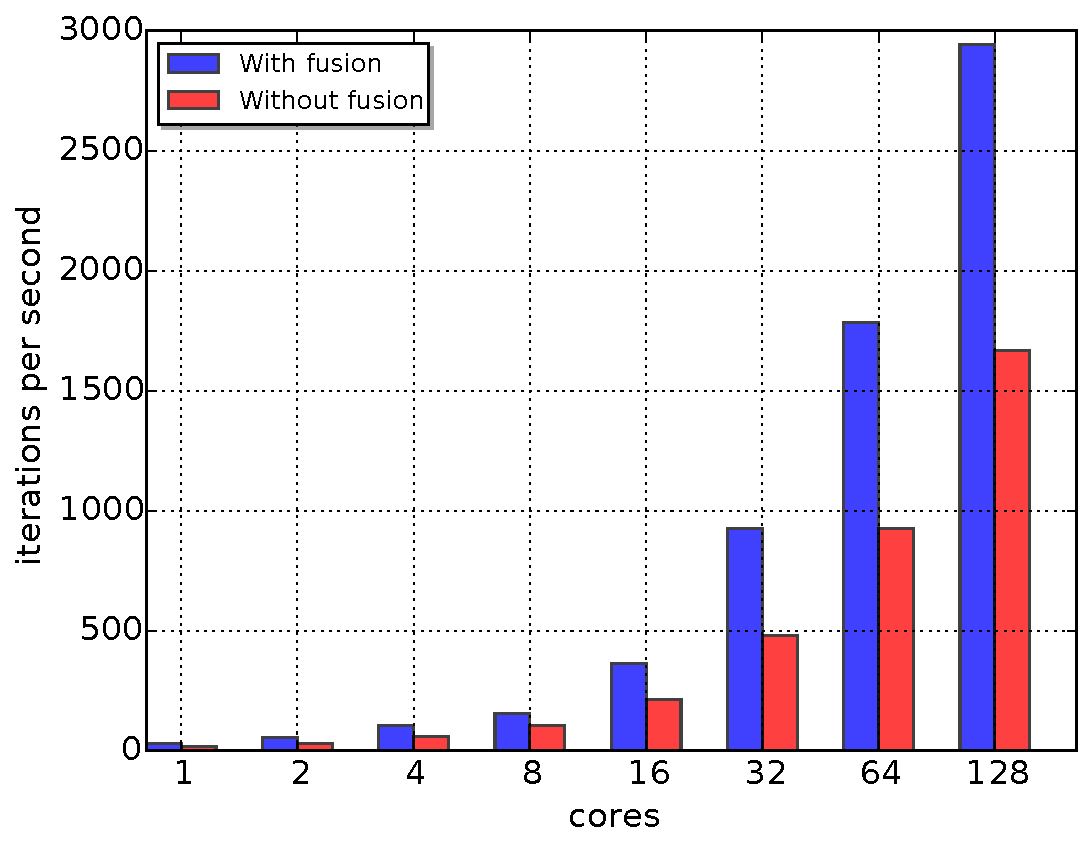
\includegraphics[width=.6\textwidth]{../results/task_scaling/500_200/fusVSbase.pdf}
%  \caption{Strong scaling on a 500x500 domain size with $200$ time iterations, with and without fusions proposed by MSF.}
%  \label{fig:fusion}
%\end{center}\end{figure}
%
%\HC{another benchmark with and without fusion fro task parallelization ?}

%-------------------------------------
\subsection{Hybrid parallelism evaluation}

In this section, we introduce task parallelism to evaluate the hybrid parallelization offered by MSF. The MSF implementation evaluated in this paper relies on SkelGIS and OpenMP.

The series-parallel tree decomposition $TSP$ of this simulation, extracted by MSC, is composed of 17 nodes labeled as sequence $\mathcal{S}$ and 18 nodes labeled as parallel $\mathcal{P}$. 

We define the \emph{level of parallelism} as the number of parallel tasks inside one fork of the fork/join model. The fork/join model obtained for FullSWOF2D is composed of 18 fork phases (corresponding to $\mathcal{P}$ nodes of $TSP$). Table~\ref{fig:freq} represents the number of time a given level of parallelism is obtained inside fork phases.

\begin{table}[th]
 \begin{center}
 \begin{tabular}{|c|c|c|c|c|c|c|c|c|}
   Level & 1 & 2 & 3 & 4 & 6 & 10 & 12 & 16\\
   \hline
   Frequency & 2 & 1 & 3 & 5 & 3 & 1 & 1 & 2\\
 \end{tabular}
\caption{Parallelism level (number of parallel tasks) and the number of times this level appears.}
\label{fig:freq}
 \end{center}
\end{table}

One can notice that the level of task parallelism extracted from the Shallow water equations is limited by two sequential parts in the application (level 1). Moreover, a level of 16~parallel tasks is reached two times, and five times for the fourth level.
This means that if two cores are dedicated to task parallelism, the two sequential parts of the code will not take advantage of these two cores, and that no part of the code would benefit from more than 16 cores. The task parallelism, as proposed in this paper (\ie where each kernel is a task) is therefore not insufficient to take advantage of a single node of modern clusters that typically supports more than 16 cores.

\begin{figure}[bh]\begin{center}
  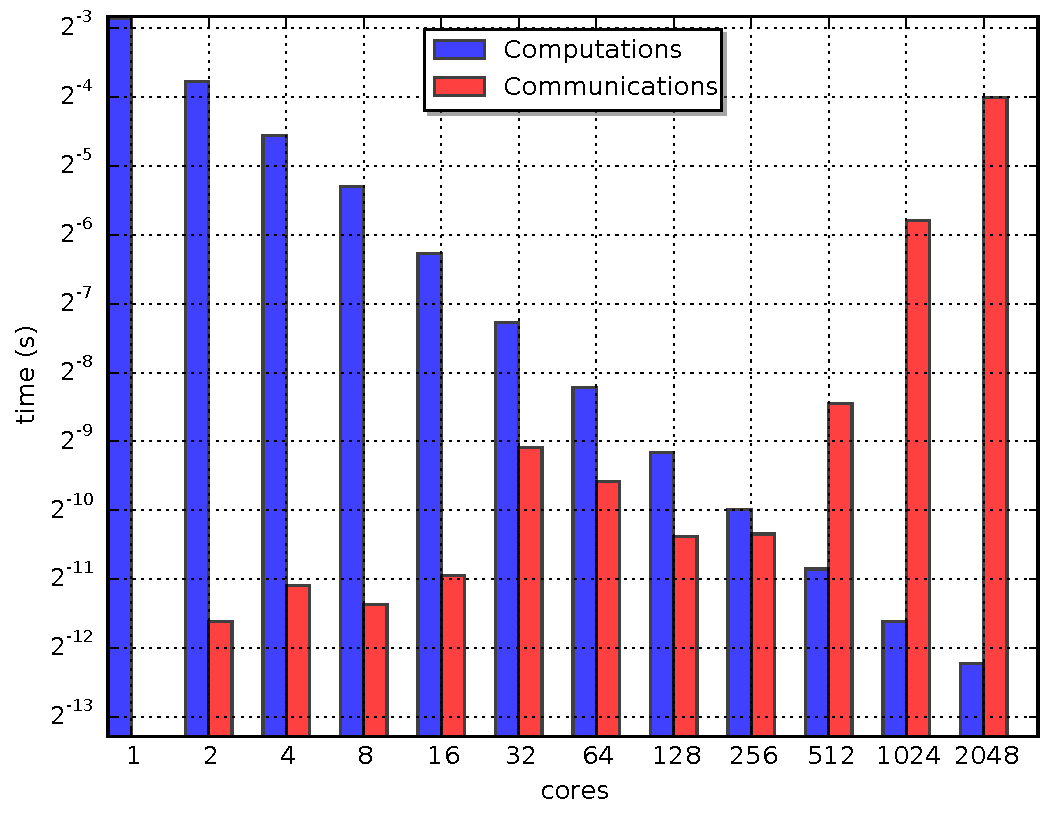
\includegraphics[width=.6\textwidth]{../results/task_scaling/500_200/analytic/times.pdf}
  \caption{Computation vs communication times in the data parallelization technique.}
  \label{fig:limit}
\end{center}\end{figure}

On the other hand, Fig.~\ref{fig:limit} illustrates limitations of data parallelization technique alone. In this figure is represented the execution time (with a logarithmic scale) of FullSWOF2D while increasing the number of cores for a fix domain size of $500 \times 500$ with a total of $200$ time iterations (\ie this is a strong scaling). The speedup of this same benchmark is represented in blue in Fig.~\ref{fig:close}. One can note that the scaling is not as good is the one presented in Fig.~\ref{fig:strong}. 
The main difference between these two benchmarks is the domain size. In the benchmark of Fig.~\ref{fig:strong} the domain size is $10k \times 10k$ which means that using $2^8$ cores, for example, each core has to compute only a $31 \times 31$ sub-domain. On the other hand using $2^8$ cores in Fig.~\ref{fig:close} each core has to compute a $625 \times 625$ sub-domain. Fig.~\ref{fig:limit} shows why the speedup is not as good as the one with a bigger domain size.  

Actually, in this figure, while the computation time (in blue) decreases linearly with the number of core used, the communication behavior (in red) is much more erratic. Between 2 and 16 cores, communications are performed inside a single node thus the time is small and nearly constant. There is a small oscillation that might be explained by the partitioning differences. SkelGIS performs a two dimensional partitioning strategy. For this reason a smaller number of bytes are communicated using 2 cores than using 4, and using 8 cores than using 16 cores. Starting from 32 cores, each node is fully used and more than one node is used. From this point thus the communication time is typically modeled as $L+S/B$ where $L$ is the latency, $S$ the data size and $B$ the bandwidth. This explains the decrease of time from 32 to 128 cores where the data sizes communicated by each process decreases. The increased observed after$128$ cores that might be due to the fact that with the increased number of processes the fat-tree becomes deeper and the latencies increase.

\begin{figure}[th]\begin{center}
  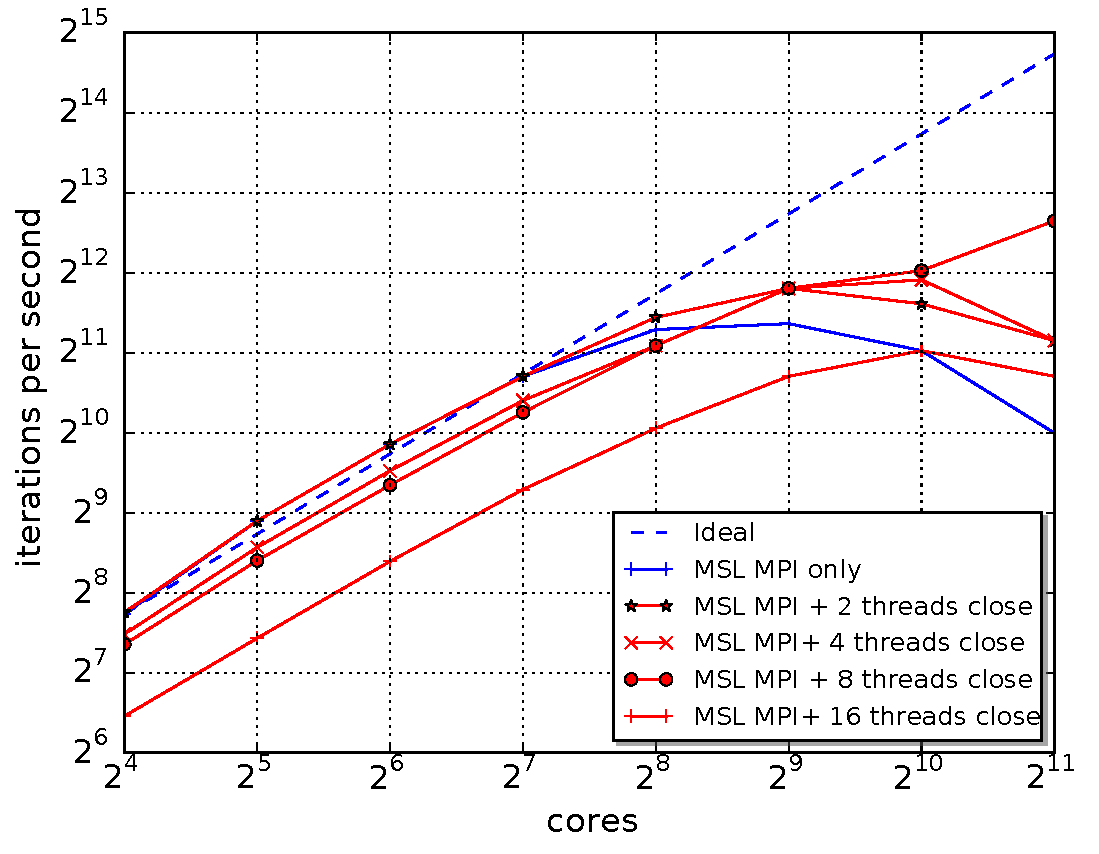
\includegraphics[width=.6\textwidth]{../results/task_scaling/500_200/base_close_median.pdf}
  \caption{Strong scaling comparisons between data parallelization and hybrid parallelization. A \emph{close} OpenMP clause is used to bind threads onto cores.}
  \label{fig:close}
\end{center}\end{figure}

All in all, when the number of core used increases, the computation/communication ratio becomes poorer and poorer. As a result, the data parallelism alone fails to provide enough parallelism to leverage the whole machine and other sources of parallelism have to be found. As expected, in  Figure~\ref{fig:close} the speedup bends down from 256 to 2048 cores. The same problem would happened in previous experiment of Fig.~\ref{fig:strong}, however as the domain size is larger, the phenomena appears with much more cores. 

As task parallelism fails to scale from 16 cores, and as data parallelism also fails to scale when the communication cost overpass the execution time, an hybrid parallelization strategy is proposed by MSF and evaluated below.

In addition to the blue curve, Fig.~\ref{fig:close} shows speedups for the same example ($500 \times 500$ domain with $200$ iterations) but using an hybrid parallelization. Fig.~\ref{fig:close} shows a comparison with 2, 4, 8 and 16 cores per MPI process for task parallelization.

For example, the purple curve shows the parallelization which uses for each data parallelization process (\ie MPI process) 8 additional cores for task parallelization. As a result, for example, when using 2 machines of the TGCC cluster, with a total of 32 cores, 4 cores are used for SkelGIS MPI processes, for data parallelization, and for each one 8 cores are used for task parallelization ($4 \times 8 = 32$). This respect $P = P_{data} \times P_{task}$ presented in Section~\ref{sect:perfs}.
As a result, and as explained in Section~\ref{sect:perfs}, quantities are less divided into sub-domains, that are responsible for communications, and the effect which is observe onto the blue curve is delayed.

From 2 to 8 cores, the improvement of the strong scaling is clear. However, reaching 16 cores, an important initial overhead appears and in addition to this, the curve bends down rapidly instead of improving the one with 8 cores for task parallelization. Two different phenomena happen in this case.

First, thin nodes of the TGCC Curie are built with two NUMA nodes each of 8 cores. As a result, when increasing the number of OpenMP cores for task parallelization from 8 to 16 cores, an overhead is introduced by exchanges of data between memories of the two NUMA nodes. This phenomena is illutrated in Fig.~\ref{fig:spread}. In this figure, a different binding strategy is used. A binding strategy is the way the scheduler binds threads onto available cores. The strategy used in Fig.~\ref{fig:spread} is called \emph{spread} (instead of \emph{close} in Figure~\ref{fig:close}). This strategy binds threads on cores in order to spread as much as possible onto resources, which means that the two NUMA nodes are directly used whatever the number of cores used for task parallelism. As a result, and as shown in the figure, using 2, 4 and 8 cores an initial overhead is introduced as the one observed in Fig.~\ref{fig:close}. This shows that the initial overhead with 16 cores is due to NUMA effects.

\begin{figure}[!h]\begin{center}
  \resizebox{8cm}{!}{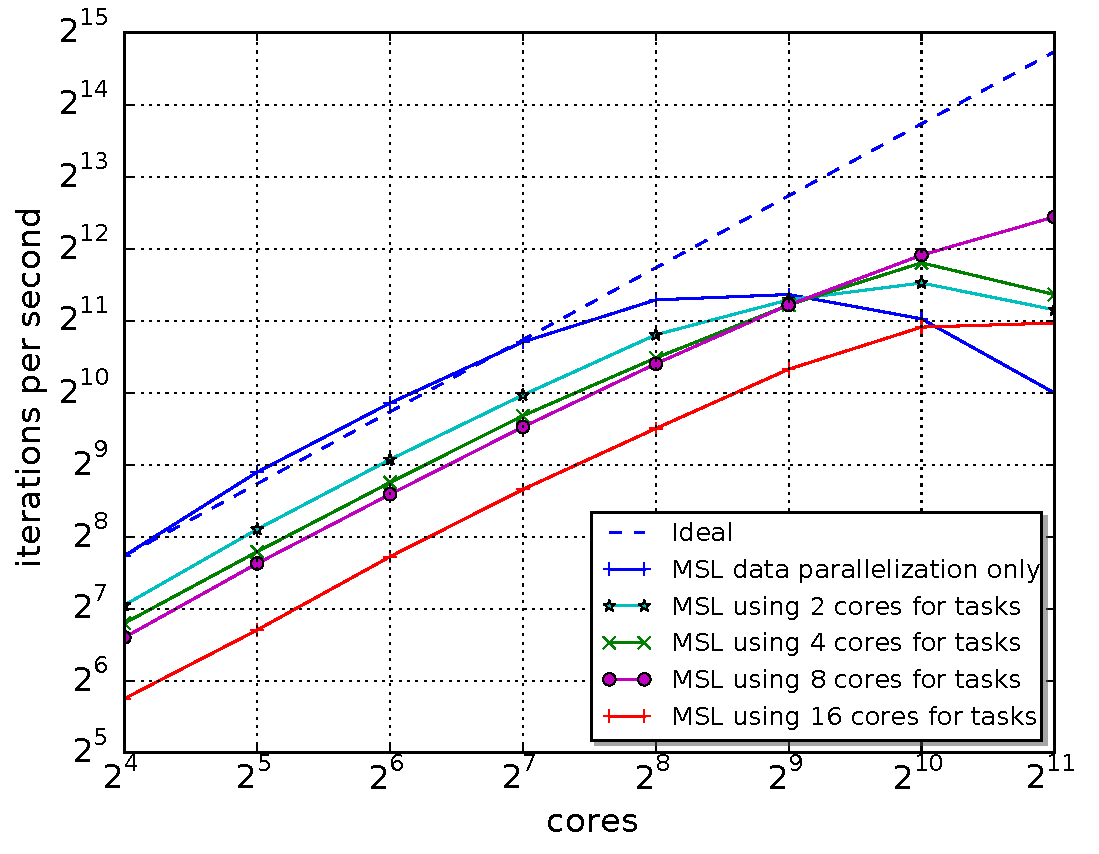
\includegraphics{../results/task_scaling/500_200/base_spread_median.pdf}}
  \caption{Strong scaling comparisons between data parallelization and hybrid parallelization. A \emph{spread} OpenMP clause is used to bind threads onto cores.}
  \label{fig:spread}
\end{center}\end{figure}

The second phenomena that happens in Figure~\ref{fig:close} using 16 cores is due to the level of parallelism introduced by the task parallelization technique. Actually, as illustrated in Table~\ref{fig:freq}, only two forks of $TSP$ can take advantage of 16 cores among a total of 18 forks. This phenomena has been mentioned in Section~\ref{sect:perfs} by the variable $F_{task}$ and the fact that it is not always true that $F_{task}=P_{task}$. This explains why using 16 cores is less efficient than using 8 cores, even when the two NUMA nodes are always used as in Fig.~\ref{fig:spread}.

Finally, to validate the performance model introduced in Section~\ref{sect:perfs}, and to understand when the hybrid parallelization becomes more interesting than the data parallelization, Figure~\ref{fig:tth2} represents $T_{COM1}$ and $T_{COM2}+T_{task}$ of Equation~(\ref{eq:hyb}), for the best case, \ie when 8 cores are used in Fig.~\ref{fig:close}.  Figure~\ref{fig:tth2} and Table~\ref{fig:tth} presents results of these measurements. Results perfectly matches Fig.~\ref{fig:close} for 8 cores per MPI process. As a result, the hybrid parallelization becomes better with a total of 512 cores in this case.

\begin{table}[!h]
 \begin{center}
 \begin{tabular}{|c|c|c|c|c|}
    \hline 
    & $T_{COM1}$ & $T_{COM2}$ & $T_{task}$ & Equation~(\ref{eq:hyb})\\
   \hline
   16 cores ($2 \times 8$) & 0.0005 & 0.00032 & 0.013 & False\\
   32 cores ($4 \times 8$) & 0.0018 & 0.00045 & 0.0062 & False\\
   64 cores ($8 \times 8$) & 0.0013 & 0.00038 & 0.0034 & False\\
   128 cores ($16 \times 8$) & 0.00075 & 0.0005 & 0.0023 & False\\
   256 cores ($32 \times 8$) & 0.00077 & 0.0018 & 0.001 & False\\
   512 cores ($64 \times 8$) & 0.0029 & 0.0013 & 0.00052 & True\\
   1024 cores ($128 \times 8$) & 0.018 & 0.00075 & 0.00029 & True\\
   2048 cores ($256 \times 8$) & 0.0623 & 0.00077 & 0.00016 & True\\
   \hline
 \end{tabular}
\caption{Execution times (seconds) of $T_{COM1}$, $T_{COM2}$ and $T_{task}$ for 8 cores for task parallelization. Verification of the Equation~(\ref{eq:hyb}).}
\label{fig:tth}
 \end{center}
\end{table}

\begin{figure}[!h]\begin{center}
  \resizebox{8cm}{!}{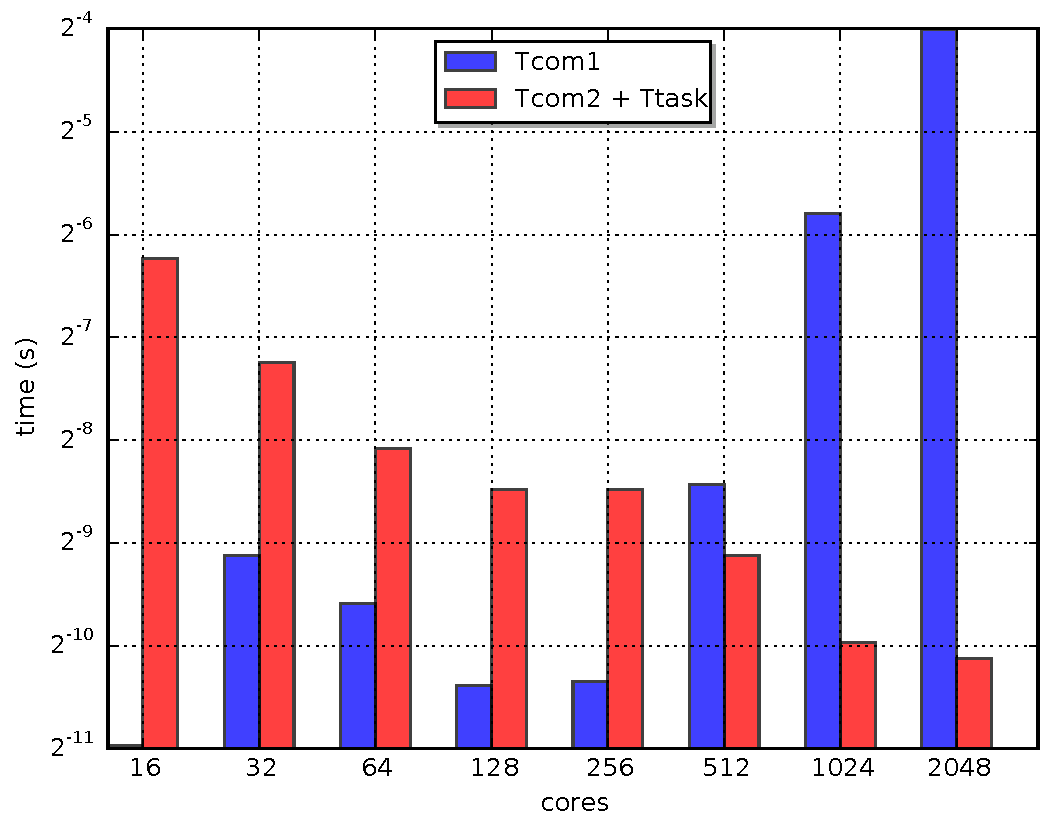
\includegraphics{../results/task_scaling/500_200/analytic/tth.pdf}}
  \caption{Execution times (seconds) of $T_{COM1}$ and $T_{COM2} + T_{task}$ for 8 cores for task parallelization. Verification of the Equation~(\ref{eq:hyb}).}
  \label{fig:tth2}
\end{center}\end{figure}

%-------------------------------------------------
\subsection{Fusion evaluation}
\label{sect:fus}
%-------------------------------------------------

\HC{under modification}

\paragraph{\textbf{Fusion}} Finally, we evaluate loop fusions automatically proposed by MSF from the $TSP$ tree of computation kernels. Figure~\ref{fig:fusion} shows the number of iterations per second as a function of the number of cores with and without fusions. This benchmark is performed on FullSWOF2D onto a $500 \times 500$ domain size with $200$ time iterations. As explained in Section~\ref{sect:fusion}, the MSF loop fusion happens at a high level and is most of the time done naturally by a computer scientist. However, for a non computer scientist which write its numerical codes, an automatic proposition of such fusions avoid errors, particularly for a parallel execution. Moreover, one can notice that the performance is clearly improved (around 40\%) by this fusion.

\begin{figure}[!h]\begin{center}
  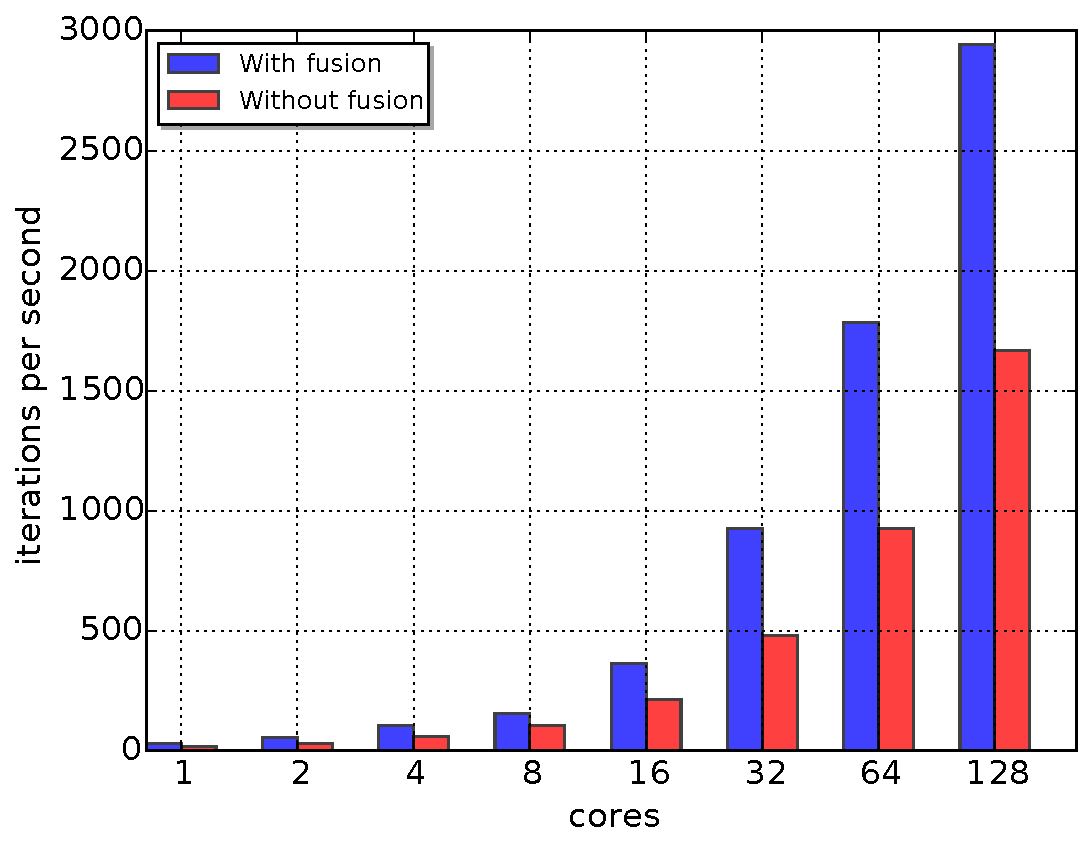
\includegraphics[width=.6\textwidth]{../results/task_scaling/500_200/fusVSbase.pdf}
  \caption{Strong scaling on a 500x500 domain size with $200$ time iterations, with and without fusions proposed by MSF.}
  \label{fig:fusion}
\end{center}\end{figure}

\begin{figure}[!h]\begin{center}
  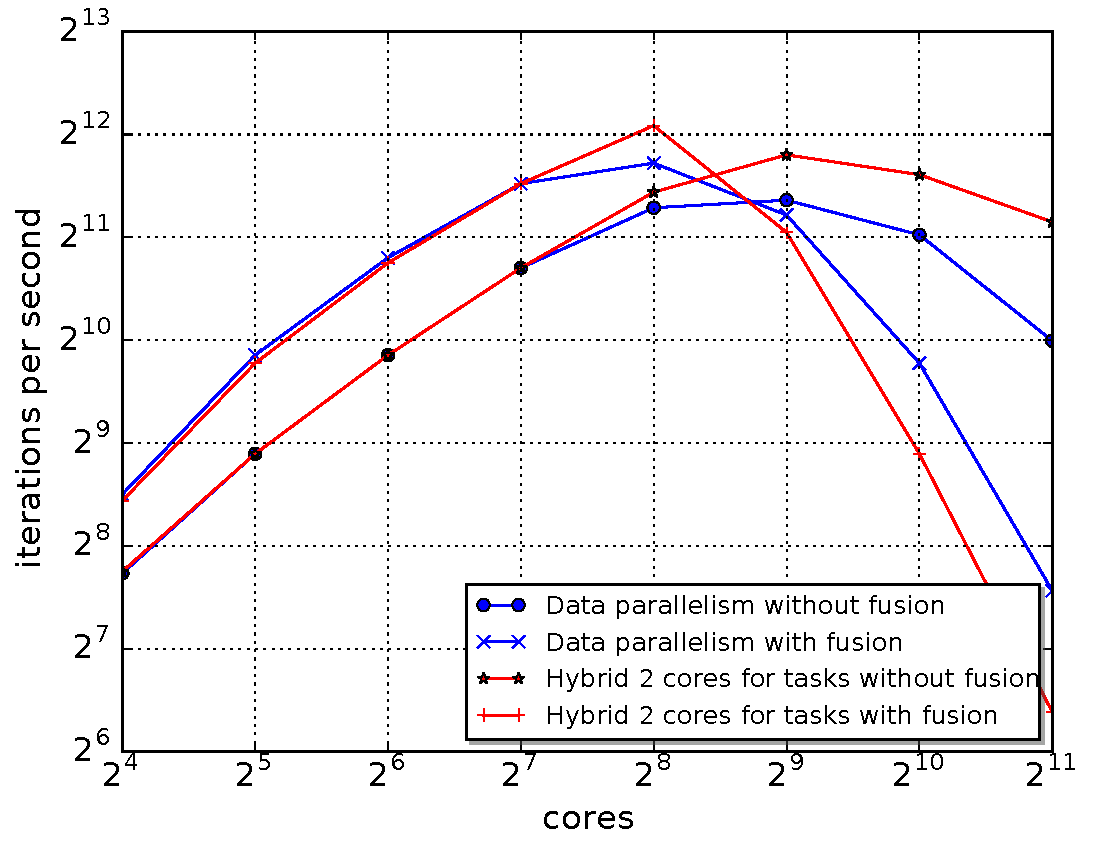
\includegraphics[width=.6\textwidth]{../results/task_scaling/500_200/withwithout2_close_median.pdf}
  \caption{blabla}
  \label{fig:fusion1}
\end{center}\end{figure}

\begin{figure}[!h]\begin{center}
  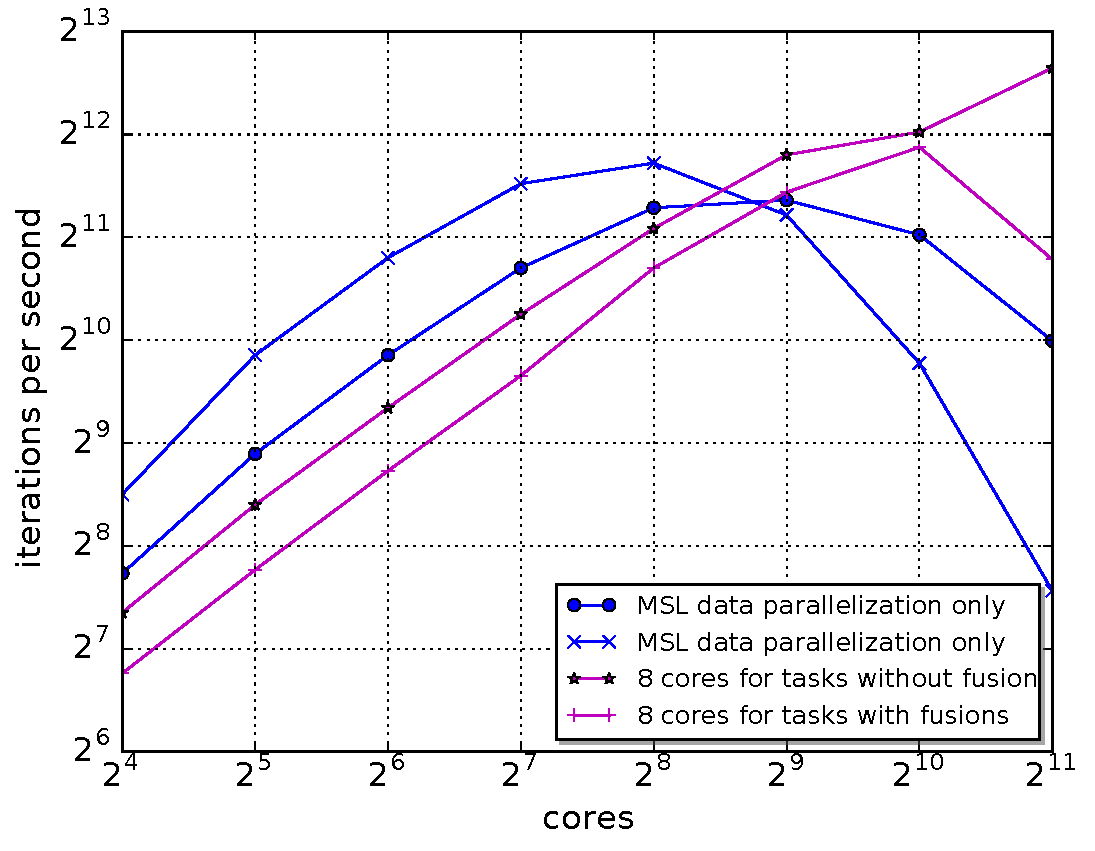
\includegraphics[width=.6\textwidth]{../results/task_scaling/500_200/withwithout8_close_median.pdf}
  \caption{blabla}
  \label{fig:fusion2}
\end{center}\end{figure}